\documentclass[11pt]{article}

\usepackage[utf8]{inputenc}
\usepackage[a4paper]{geometry}
\usepackage{graphicx}
\usepackage{enumitem}
\usepackage{caption}
\usepackage{hyperref}

\graphicspath{ {./figures/} }

\setlength{\parindent}{0em}
\setlength{\parskip}{0.5em}

\title{ILP Coursework 2 Report}
\author{Angus Stewart (s1902147)}
\date{December 2020}

\begin{document}

\maketitle

\tableofcontents

%%%
\newpage
\newgeometry{left=1.5cm, right=1.5cm, top=2cm, bottom=2cm}
%%%

\section{Software Architecture}

\newpage

\section{Drone Control Algorithm}
The specification document describes a modified version of the well known \href{https://en.wikipedia.org/wiki/Travelling\_salesman\_problem}{travelling salesman problem} (TSP) where we look to visit each sensor and return to the starting position. Of course, it is not exactly the same problem as the path to each sensor is not a single link but rather a series of restricted movements. Hence, the combination of the travelling salesman problem being NP-complete and the movements of the drone made the complexity of the problem very apparent from the beginning.

Knowing that finding an algorithm that would solve the entire path planning problem optimally would not be feasible, I broke the problem into two sub-problems. The first is the order in which the drone visits the sensors and the second is finding the sequence of valid moves to get from one coordinate position to another.

With these two components, we can find the entire route:
\begin{enumerate}[topsep=0pt, itemsep=0pt]
    \item Get the next \textbf{unvisited} sensor given the current position of the drone
    \item Find the route to the sensor
    \begin{enumerate}[topsep=0pt, itemsep=0pt]
        \item If enough battery, move the drone along the route and mark the sensor as visited
        \item Otherwise, skip to step 4
    \end{enumerate}
    \item Go to step 1 until all sensors have been visited
    \item Find the route back to the start given the current position. If not enough battery to complete the entire route, follow the route until we run out of battery to return as close to the start as possible.
\end{enumerate}


\begin{figure}[h]
    \centering
    \begin{minipage}{0.5\textwidth}
        \centering
        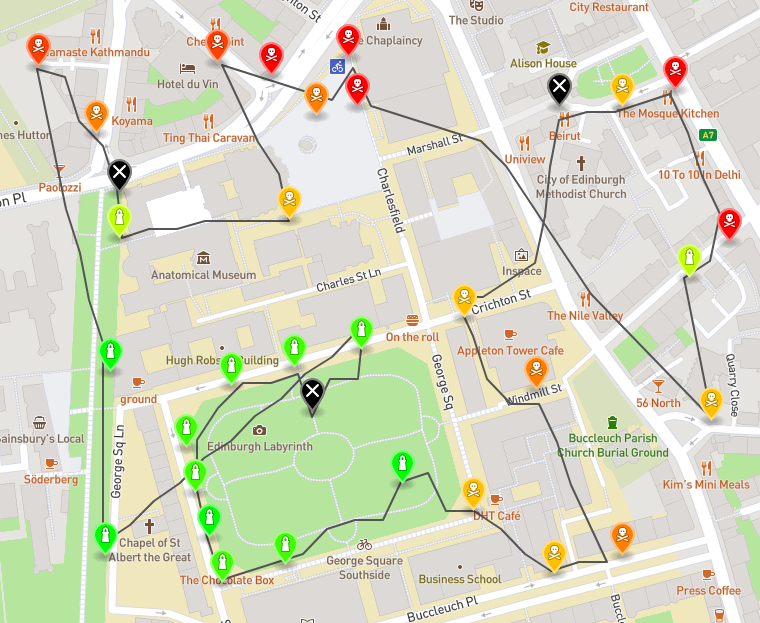
\includegraphics[width=0.95\textwidth, height=16em]{25-10-2021}
        \captionof{figure}{25th of October 2021}
        \label{fig:example1}
    \end{minipage}%
    \begin{minipage}{0.5\textwidth}
        \centering
        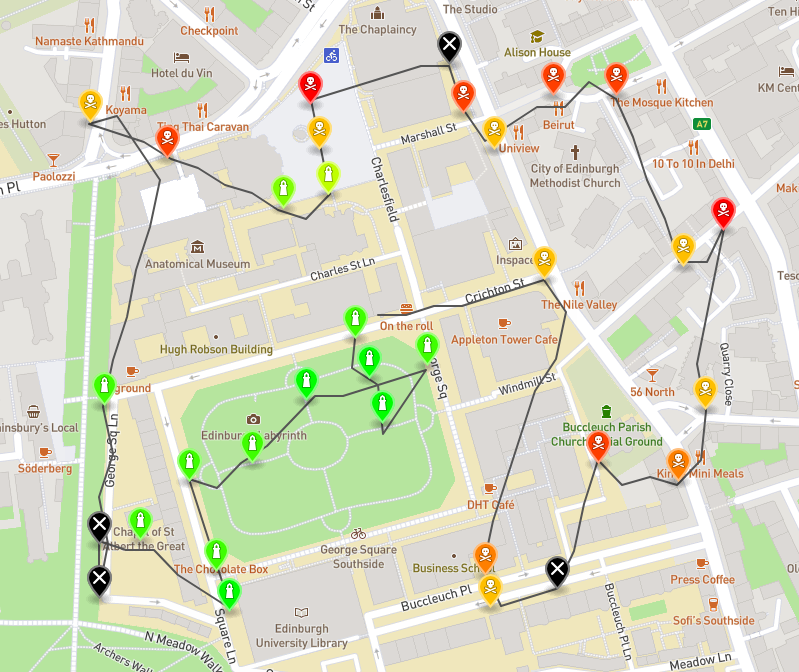
\includegraphics[width=0.95\textwidth, height=16em]{26-12-2021}
        \captionof{figure}{26th of December 2021}
        \label{fig:example2}
    \end{minipage}
\end{figure}

\subsection{Ordering of the Sensors}
The first problem is determining the order in which the drone should visit the sensors. To keep things simple, I chose a greedy approach, and this is what the drone uses in the implementation. The algorithm calculates the straight-line distance between a given coordinate position (e.g. current position of the drone) and the coordinates of a list of sensors (e.g. list of unvisited sensors) and returns the closest sensor.

Although this algorithm is simple and runs very quickly (linear in the number of sensors), it is unlikely to produce an optimal sequence of sensors to visit. We can see this with Figure \ref{fig:example1} where the drone has to take long routes across the map to reach sensors that it missed. In addition, it does not take into account the no-fly-zones of the map and how this affects the distances between sensors. But given the TSP nature of this problem, obtaining good solutions requires significant effort in implementing complex algorithms. Hence, I believe this greedy algorithm is a good starting point due to its balance of simplicity and performance.

It is worth noting that the drone only looks for the next sensor and does not pre-compute the order of all sensors. This decision was taken because the drone does not necessarily reach the exact coordinates of the target sensor and hence pre-computing everything from the beginning would be inaccurate.



\subsection{Routing to the Next Position}
Given the current position of the drone and the target position (e.g coordinates of the next sensor or of the starting position), we must calculate a valid route between the two points. Note that we do not need to end up \textbf{at} the target position, just within a certain distance from it (e.g 0.0002 for sensors).

This can be thought of as a tree search problem. The tree represents all possible sequences of moves (represented by the edges of the tree) that the drone is allowed to make, and the nodes represents coordinate positions with the root being the current position of the drone. Note that the branching factor for this tree is 36 (though it may be less if the movement of the drone is restricted e.g due to being near no-fly-zones).

In my implementation, I use a modified A* search algorithm to find the path down the tree to a node that is within range of our target position. The algorithm consists of two lists: \texttt{closedPathPoints}, which stores all the nodes that we have visited (expanded) and \texttt{openPathPoints}, which stores all the nodes that we have yet to visit but whose parents have been visited.
\begin{enumerate}[topsep=0pt, itemsep=0pt]
  \item We begin with only the root node in \texttt{openPathPoints}. Remove this node from the list and 'expand' it to generate all its children nodes. These children nodes represent \textbf{valid} positions one step away from the current node.
  \begin{enumerate}[topsep=0pt, itemsep=0pt]
      \item Each child node gets assigned a \texttt{distanceScore} (among other attributes such as \texttt{prev}) which is the sum of the travelled distance from the root to the current node and the straight-line distance from the current node to the target position.
      \item We then select 5 of the child nodes with the smallest \texttt{distanceScore}. We do this to reduce the time complexity of the algorithm as using all child nodes would cause the algorithm to run slowly.
  \end{enumerate}
  
  \item Add the 5 nodes to \texttt{openPathPoints} and add the root to \texttt{closedPathPoints}
  
  \item Select the node from \texttt{openPathPoints} with the lowest \texttt{distanceScore}. If in range of the target position, skip to step 6, otherwise expand it as per step 1.
  
  \item Before adding each of the 5 nodes to \texttt{openPathPoints}, we do two checks:
  \begin{enumerate}[topsep=0pt, itemsep=0pt]
      \item If their coordinates match with a node already in \texttt{openPathPoints}, we look to see if it has a smaller \texttt{distanceScore}. If it does, we add the new node and remove the old one. Otherwise, we discard the new node.
      \item If the node was not added to \texttt{openPathPoints} or discarded in part (a), check to see if the coordinates match with a node already in \texttt{closedPathPoints}. If it does, discard the node.      
    \end{enumerate}   
    
  \item Add the expanded node (from step 3) to \texttt{closedPathPoints} and go to step 3

  \item Reconstruct the route from the final node from step 3 by following \texttt{prev} (which points to the node's parent) until we reach the root.
\end{enumerate}

Notice that this algorithm will always produce a route of at least length 1 because it always expands the root node before checking if any of the nodes are within range of the target position. This is required as per the specification. However, because we do not need to move before finishing, when calculating the route back to the start we check before step 1 whether the root is within range of the target position.

This algorithm has the advantage that it can handle no-fly-zones without much modification (we just don't generate the child nodes that cross the no-fly-zones). This contrasts with my original algorithm that used a greedy approach which would get `stuck' oscillating between two nodes if the target position was on the other side of a no-fly-zone. This is because unlike the A* search algorithm, the greedy algorithm did not take into account the distance from the root node. However, the time complexity of the A* algorithm is not as good (hence step 1.b) so the time the algorithm takes to find routes over larger distances become much more noticeable which puts the scalability of this algorithm into question.

It is also worth mentioning here, that although \textbf{the algorithm is the same}, in the actual implementation we use \texttt{PathPoint} objects, which represent the movement of the drone and hence would correspond to the edges of the tree, rather than nodes as described above. However, \texttt{PathPoint} stores the nodes in \texttt{endPos} (and its parent in \texttt{startPos}) and attributes such as \texttt{distanceScore} correspond to the position of \texttt{endPos} and so the implementation details of the algorithm is very similar.

\newpage

\section{Class Documentation}


\newpage

\section{References}
The following sources were used either to provide inspiration for my implementation or to directly aid in it (e.g. through example code or pseudocode):
\begin{enumerate}
    \item \href{https://en.wikipedia.org/wiki/Motion_planning#Grid-based_search}{Wikipedia - Motion Planning}
    \item \href{https://en.wikipedia.org/wiki/Any-angle_path_planning}{Wikipedia - Any-angle Path Planning}
    \item \href{https://en.wikipedia.org/wiki/A*_search_algorithm#}{Wikipedia - A* Search Algorithm}
    \item \href{https://en.wikipedia.org/wiki/Best-first_search}{Wikipedia - Best First Search}
    \item \href{https://stackoverflow.com/questions/16069106/how-to-compare-two-java-objects}{Stackoverflow - How to Compare Two Java Objects}
\end{enumerate}

\end{document}
